\documentclass[12pt]{article}
\usepackage{../../ficha}

\begin{document}

\ficha{Lei dos Senos e Lei dos Cossenos}[Resolução de Triângulos Quaisquer]

\instrucoes{Num triângulo $ABC$, $a$, $b$ e $c$ são os lados opostos aos ângulos $A$, $B$ e $C$. Lei dos senos: $\dfrac{\sin A}{a} = \dfrac{\sin B}{b} = \dfrac{\sin C}{c}$. Lei dos cossenos: $a^2 = b^2 + c^2 - 2bc\cos A$. Podes usar calculadora; arredonda às centésimas.}

\begin{center}
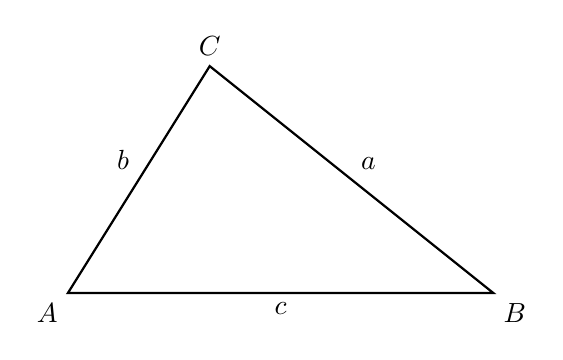
\begin{tikzpicture}[scale=0.9]
  \coordinate (A) at (0,0); \coordinate (B) at (6,0); \coordinate (C) at (2,3.2);
  \draw[thick] (A) node[below left] {$A$} -- (B) node[below right] {$B$} -- (C) node[above] {$C$} -- cycle;
  \node[below] at (3,0) {$c$}; \node[above right] at (4,1.6) {$a$}; \node[above left] at (1,1.6) {$b$};
\end{tikzpicture}
\end{center}

\secao{Revisão: Razões Trigonométricas}{Resolve.}
\begin{exercicios}
  \item Indica os valores exatos de $\sin 30^\circ$, $\cos 45^\circ$ e $\tan 60^\circ$.
  \item Sabendo que $\sin \alpha = \dfrac{3}{5}$ e $\alpha$ é agudo, determina $\cos \alpha$ e $\tan \alpha$.
  \item Sabendo que $\tan \alpha = 2$ e $\alpha$ é agudo, determina $\cos \alpha$.
  \item Mostra que $\sin^2 \alpha + \cos^2 \alpha = 1$ usando um triângulo retângulo.
  \item Indica $\sin 150^\circ$ e $\cos 120^\circ$ (valores exatos).
  \item Num triângulo retângulo, a hipotenusa mede 10 e um ângulo agudo mede $35^\circ$. Calcula os catetos.
\end{exercicios}

\secao{Lei dos Senos}{Resolve o triângulo (determina os elementos desconhecidos).}
\begin{exercicios}
  \item $A = 40^\circ$, $B = 60^\circ$, $a = 8$.
  \item $A = 35^\circ$, $C = 75^\circ$, $b = 12$.
  \item $B = 45^\circ$, $C = 30^\circ$, $c = 10$ (valores exatos).
  \item $A = 120^\circ$, $B = 25^\circ$, $c = 15$.
  \item $A = 50^\circ$, $a = 10$, $b = 12$. (Atenção: pode haver duas soluções.)
  \item $A = 30^\circ$, $a = 5$, $b = 10$. Que tipo de triângulo é?
  \item $A = 30^\circ$, $a = 3$, $b = 10$. Existe triângulo?
\end{exercicios}

\secao{Lei dos Cossenos}{Resolve o triângulo.}
\begin{exercicios}
  \item $b = 5$, $c = 8$, $A = 60^\circ$ (calcula $a$ exatamente).
  \item $a = 7$, $b = 10$, $C = 45^\circ$.
  \item $a = 12$, $c = 9$, $B = 110^\circ$.
  \item $a = 5$, $b = 7$, $c = 8$ (determina os três ângulos).
  \item $a = 3$, $b = 5$, $c = 7$ (determina o maior ângulo exatamente).
  \item $a = 6$, $b = 6$, $c = 6\sqrt{2}$. Que tipo de triângulo é?
  \item Usando a lei dos cossenos, mostra que, se $C = 90^\circ$, se obtém o Teorema de Pitágoras.
\end{exercicios}

\secao{Área de Triângulos}{Calcula a área, usando $\text{Área} = \dfrac{1}{2}\,ab\sin C$.}
\begin{exercicios}
  \item $a = 6$, $b = 8$, $C = 30^\circ$.
  \item $a = 10$, $c = 7$, $B = 120^\circ$ (valor exato).
  \item $b = 5$, $c = 9$, $A = 75^\circ$.
  \item Um triângulo equilátero de lado 4 (valor exato).
  \item $a = 5$, $b = 7$, $c = 8$ (determina primeiro um ângulo).
\end{exercicios}

\secao{Problemas}{Resolve.}
\begin{exercicios}
  \item Dois barcos partem do mesmo porto em direções que formam $70^\circ$. Ao fim de uma hora, um percorreu 15\,km e o outro 20\,km. A que distância estão um do outro?
  \item Para medir a largura de um rio, marcaram-se dois pontos $A$ e $B$ numa margem, a 50\,m um do outro, e um ponto $C$ na outra margem. Mediu-se $C\hat{A}B = 62^\circ$ e $C\hat{B}A = 71^\circ$. Calcula $AC$ e a largura do rio.
  \item Um terreno triangular tem lados de 40\,m, 55\,m e 70\,m. Calcula o maior ângulo e a área do terreno.
  \item Do topo de um farol, com 30\,m de altura, avista-se um barco com um ângulo de depressão de $12^\circ$. A que distância da base do farol está o barco?
  \item Um paralelogramo tem lados de 6\,cm e 10\,cm e um ângulo de $50^\circ$. Calcula o comprimento das duas diagonais.
\end{exercicios}

\secao{Desafios}{Resolve os problemas.}
\begin{exercicios}
  \item Prova a lei dos senos a partir da fórmula da área $\dfrac{1}{2}ab\sin C = \dfrac{1}{2}bc\sin A = \dfrac{1}{2}ac\sin B$.
  \item Num triângulo, $a = 2b$ e $C = 60^\circ$. Mostra que o triângulo é retângulo e indica qual o ângulo reto.
  \item Mostra que o raio $R$ da circunferência circunscrita verifica $\dfrac{a}{\sin A} = 2R$.
  \item Dois observadores, a 200\,m um do outro, veem um balão com ângulos de elevação de $40^\circ$ e $55^\circ$ (o balão está entre os dois, no mesmo plano vertical). A que altura está o balão?
\end{exercicios}

\end{document}
